\section{Special relativity}
When particles move Extremely Fast\textsuperscript{TM}, Newtonian Dynamics becomes inaccurate and is replaced by Einstein's Special Theory of Relativity (1905).

Its effects are noticeable only when particles approach to the speed of light,
\[
  c = 299792458 \rmm\rms^{-1} \approx 3e8\rmm\rms^{-1}.
\]
This is \emph{really fast}.

The Special Theory of Relativity rests on the following postulate:
\begin{center}
  \emph{The laws of physics are the same in all inertial frames}
\end{center}
This is the principle of relativity familiar to Galileo. Galilean relativity mentioned in the first chapter satisfies this postulate for dynamics. People then thought that Galilean relativity is what the world obeys. However, it turns out that there is a whole family of solutions that satisfy the postulate (for dynamics), and Galilean relativity is just one of them.

This is not a problem (yet), since Galilean relativity seems so intuitive, and we might as well take it to be the true one. However, it turns out that solving Maxwell's equations of electromagnetism gives an explicit value of the speed of light, $c$. This is independent of the frame of reference. So the speed of light must be the same in every inertial frame.

This is not compatible with Galilean relativity.

Consider the two inertial frames $S$ and $S'$, moving with relative velocity $v$. Then if light has velocity $c$ in $S$, then Galilean relativity predicts it has velocity $c - v$ in $S'$, which is wrong.

Therefore, we need to find a different solution to the principle of relativity that preserves the speed of light.

\subsection{The Lorentz transformation}
Consider again inertial frames $S$ and $S'$ whose origins coincide at $t = t' = 0$. For now, neglect the $y$ and $z$ directions, and consider the relationship between $(x, t)$ and $(x', t')$. The general form is
\[
  x' = f(x, t),\quad t' = g(x, t),
\]
for some functions $f$ and $g$. This is not very helpful.

In any inertial frame, a free particle moves with constant velocity. So straight lines in $(x, t)$ must map into straight lines in $(x', t')$. Therefore the relationship must be linear.

Given that the origins of $S$ and $S'$ coincide at $t = t' = 0$, and $S'$ moves with velocity $v$ relative to $S$, we know that the line $x = vt$ must map into $x'= 0$.

Combining these two information, the transformation must be of the form
\[
  x' = \gamma(x - vt),\tag{1}
\]
for some factor $\gamma$ that may depend on $|v|$ (\emph{not} $v$ itself. We can use symmetry arguments to show that $\gamma$ should take the same value for velocities $v$ and $-v$).

Note that Galilean transformation is compatible with this -- just take $\gamma$ to be always $1$.

Now reverse the roles of the frames. From the perspective $S'$, $S$ moves with velocity $-v$. A similar argument leads to
\[
  x = \gamma(x' + vt'),\tag{2}
\]
with the same factor $\gamma$, since $\gamma$ only depends on $|v|$. Now consider a light ray (or photon) passing through the origin $x = x' = 0$ at $t = t' = 0$. Its trajectory in $S$ is
\[
  x = ct.
\]
We want a $\gamma$ such that the trajectory in $S'$ is
\[
  x' = ct'
\]
as well, so that the speed of light is the same in each frame. Substitute these into (1) and (2)
\begin{align*}
  ct' &= \gamma(c - v)t\\
  ct &= \gamma(c + v)t'
\end{align*}
Multiply the two equations together and divide by $tt'$ to obtain
\[
  c^2 = \gamma^2(c^2 - v^2).
\]
So
\[
  \gamma = \sqrt{\frac{c^2}{c^2 - v^2}} = \frac{1}{\sqrt{1 - (v/c)^2}}.
\]
\begin{definition}[Lorentz factor]
  The \emph{Lorentz factor} is
  \[
    \gamma = \frac{1}{\sqrt{1 - (v/c)^2}}.
  \]
\end{definition}
Note that
\begin{itemize}
  \item $\gamma \geq 1$ and is an increasing function of $|v|$.
  \item When $v \ll c$, then $\gamma \approx 1$, and we recover the Galilean transformation.
  \item When $|v|\to c$, then $\gamma\to \infty$.
  \item If $|v| \geq c$, then $\gamma$ is imaginary, which is physically impossible (or at least \emph{weird}).
  \item If we take $c\to \infty$, then $\gamma = 1$. So Galilean transformation is the transformation we will have if light is infinitely fast. Alternatively, in the world of Special Relativity, the speed of light is ``infinitely fast''.
\end{itemize}
\begin{center}
  \begin{tikzpicture}[xscale=3, yscale=0.2]
    \draw [->] (0, 0) -- (1.1, 0) node [right] {$\frac{v}{c}$};
    \draw [->] (0, 0) -- (0, 15) node [above] {$\gamma$};
    \draw [domain=0:0.997, samples=100] plot (\x, {1 / sqrt(1 - \x * \x)});
    \draw [dashed] (1, 15) -- (1, 0) node [below] {$1$};
  \end{tikzpicture}
\end{center}
For the sense of scale, we have the following values of $\gamma$ at different speeds:
\begin{itemize}
  \item $\gamma = 2$ when $v = 0.866c$.
  \item $\gamma = 10$ when $v = 0.9949$.
  \item $\gamma = 20$ when $v = 0.999c$.
\end{itemize}

We still have to solve for the relation between $t$ and $t'$. Eliminate $x$ between (1) and (2) to obtain
\[
  x = \gamma(\gamma(x - vt) + vt').
\]
So
\[
  t' = \gamma t - (1 - \gamma^{-2})\frac{\gamma x}{v} = \gamma\left(t - \frac{v}{c^2}x\right).
\]
So we have
\begin{law}[Principle of Special Relativity]
  Let $S$ and $S'$ be inertial frames, moving at the relative velocity of $v$. Then
  \begin{align*}
    x' &= \gamma(x - vt)\\
    t' &= \gamma\left(t - \frac{v}{c^2}x\right),
  \end{align*}
  where
  \[
    \gamma = \frac{1}{\sqrt{1 - (v/c)^2}}.
  \]
  This is the \emph{Lorentz transformations} in the standard configuration (in one spatial dimension).
\end{law}
The above is the form the Lorentz transformation is usually written, and is convenient for actual calculations. However, this lacks symmetry between space and time. To display the symmetry, one approach is to use units such that $c = 1$. Then we have
\begin{align*}
  x' &= \gamma(x - vt),\\
  t' &= \gamma(t - vx).
\end{align*}
Alternatively, if we want to keep our $c$'s, instead of comparing $x$ and $t$, which have different units, we can compare $x$ and $ct$. Then we have
\begin{align*}
  x' &= \gamma\left(x - \frac{v}{c}(ct)\right),\\
  ct' &= \gamma\left(ct - \frac{v}{c}x\right).
\end{align*}
Symmetries aside, to express $x, t$ in terms of $x', t'$, we can invert this linear mapping to find (after some algebra)
\begin{align*}
  x &= \gamma(x' + vt')\\
  t &= \gamma\left(t' + \frac{v}{c^2}x'\right)
\end{align*}
Directions perpendicular to the relative motion of the frames are unaffected:
\begin{align*}
  y' &= y\\
  z' &= z
\end{align*}
Now we check that the speed of light is really invariant:

For a light ray travelling in the $x$ direction in $S$:
\[
  x = ct,\quad y = 0,\quad z = 0.
\]
In $S'$, we have
\[
  \frac{x'}{t'} = \frac{\gamma(x - vt)}{\gamma(t - vx/c^2)} = \frac{(c - v)t}{(1 - v/c)t} = c,
\]
as required.

For a light ray travelling in the $Y$ direction in $S$,
\[
  x = 0,\quad y = ct,\quad z = 0.
\]
In $S'$,
\[
  \frac{x'}{t'} = \frac{\gamma(x - vt)}{\gamma(t - vx/c^2)} = -v,
\]
and
\[
  \frac{y'}{t'} = \frac{y}{\gamma(t - vx/c^2} = \frac{c}{\gamma},
\]
and
\[
  z' = 0.
\]
So the speed of light is
\[
  \frac{\sqrt{x'^2 + y'^2}}{t'} = \sqrt{v^2 + \gamma^{-2}c^2} = c,
\]
as required.

More generally, the Lorentz transformation implies
\begin{align*}
  c^2t'^2 - r'^2 &= c^2t'^2 - x'^2 - y'^2 - z'^2\\
  &= c^2 \gamma^2\left(t - \frac{v}{c^2}x\right)^2 - \gamma^2(x - vt)^2 - y^2 - z^2\\
  &= \gamma^2\left(1 - \frac{v^2}{c^2}\right)(c^2t^2 - x^2) - y^2 - z^2\\
  &= c^2t^2 - x^2 - y^2 - z^2\\
  &= c^2t^2 - r^2.
\end{align*}
We say that the quantity $c^2t^2 - x^2 - y^2 - z^2$ is \emph{Lorentz-invariant}.

So if $\frac{r}{t} = c$, then $\frac{r'}{t'} = c$ also.

\subsection{Spacetime diagrams}
It is often helpful to plot out what is happening on a diagram. We plot them on a graph, where the position $x$ is on the horizontal axis and the time $ct$ is on the vertical axis. We use $ct$ instead of $t$ so that the dimensions make sense.
\begin{center}
  \begin{tikzpicture}[yscale=1.3]
    \draw [->] (0, 0) -- (3, 0) node [right] {$x$};
    \draw [->] (0, 0) -- (0, 2.3) node [above] {$ct$};
    \draw (0.7, 0.3) .. controls (0.7, 0.8) and (2, 1.3) .. (2, 1.8) node [right] {world line};

    \node [dot] at (1.35, 1.05) {};
    \node at (1.35, 1.05) [anchor = north west] {$P$};
  \end{tikzpicture}
\end{center}
\begin{definition}[Spacetime]
  The union of space and time in special relativity is called \emph{Minkowski spacetime}. Each point $P$ represents an \emph{event}, labelled by coordinates $(ct, x)$ (note the order!).

  A particle traces out a \emph{world line} in spacetime, which is straight if the particle moves uniformly.

  Light rays moving in the $x$ direction have world lines inclined at $45^\circ$.
  \begin{center}
    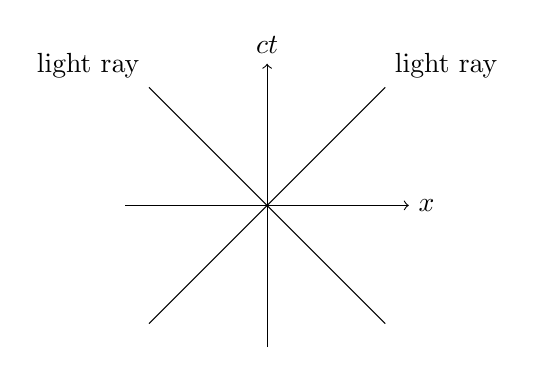
\begin{tikzpicture}[scale=0.6]
      \draw [->] (-3, 0) -- (3, 0) node [right] {$x$};
      \draw [->] (0, -3) -- (0, 3) node [above] {$ct$};
      \draw (-2.5, -2.5) -- (2.5, 2.5) node [anchor = south west] {light ray};
      \draw (2.5, -2.5) -- (-2.5, 2.5) node [anchor = south east] {light ray};
    \end{tikzpicture}
  \end{center}
\end{definition}

We can also draw the axes of $S'$, moving in the $x$ direction at velocity $v$ relative to $S$. The $ct'$ axis corresponds to $x' = 0$, i.e.\ $x = vt$. The $x'$ axis corresponds to $t' = 0$, i.e.\ $t = vx/c^2$.
\begin{center}
  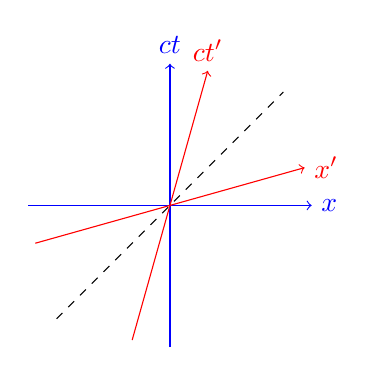
\begin{tikzpicture}[scale=0.6]
    \draw [->, blue] (-3, 0) -- (3, 0) node [right] {$x$};
    \draw [->, blue] (0, -3) -- (0, 3) node [above] {$ct$};
    \draw [->, red] (-2.85, -0.8) -- (2.85, 0.8) node [right] {$x'$};
    \draw [->, red] (-0.8, -2.85) -- (0.8, 2.85) node [above] {$ct'$};
    \draw [dashed] (-2.4, -2.4) -- (2.4, 2.4);
  \end{tikzpicture}
\end{center}
Note that the $x'$ and $ct'$ axes are \emph{not} orthogonal, but are symmetrical about the diagonal (dashed line). So they agree on where the world line of a light ray should lie on.
\subsection{Relativistic physics}
Now we can look at all sorts of relativistic weirdness!
\subsubsection*{Simultaneity}
The first relativistic weirdness is that different frames disagree on whether two evens are simultaneous
\begin{definition}[Simultaneous events]
  We say two events $P_1$ and $P_2$ are simultaneous in the frame $S$ if $t_1 = t_2$.
\end{definition}
They are represented in the following spacetime diagram by horizontal dashed lines.

However, events that are simultaneous in $S'$ have equal values of $t'$, and so lie on lines
\[
  ct - \frac{v}{c}x = \text{constant}.
\]
\begin{center}
  \begin{tikzpicture}[scale=0.6]
    \draw [->, blue] (-3, 0) -- (3, 0) node [right] {$x$};
    \draw [->, blue] (0, -3) -- (0, 3) node [above] {$ct$};
    \draw [dashed, blue] (-3, 1) -- (3, 1);
    \draw [dashed, blue] (-3, 2) -- (3, 2);
    \node [dot] at (-1.5, 2) {};
    \node [dot] at (1.5, 2) {};
    \node at (-1.5, 2) [below] {$P_1$};
    \node at (1.5, 2) [below] {$P_2$};
    \draw [->, red] (-2.85, -0.8) -- (2.85, 0.8) node [right] {$x'$};
    \draw [dashed, red] (-2.85, 0.2) -- (2.85, 1.8);
    \draw [dashed, red] (-2.85, 1.2) -- (2.85, 2.8);
    \draw [->, red] (-0.8, -2.85) -- (0.8, 2.85) node [above] {$ct'$};
  \end{tikzpicture}
\end{center}
The lines of simultaneity of $S'$ and those of $S$ are different, and events simultaneous in $S$ need not be simultaneous in $S'$. So simultaneity is relative. $S$ thinks $P_1$ and $P_2$ happened at the same time, while $S'$ thinks $P_2$ happens first.

Note that this is genuine disagreement. It is not due to effects like, it takes time for the light conveying the information to different observers. Our account above already takes that into account (since the whole discussion does not involve specific observers).

\subsubsection*{Causality}
Although different people may disagree on the temporal order of events, the consistent ordering of cause and effect can be ensured.

Since things can only travel at at most the speed of light, $P$ cannot affect $R$ if $R$ happens a millisecond after $P$ but is at millions of galaxies away. We can draw a \emph{light cone} that denotes the regions in which things can be influenced by $P$. These are the regions of space-time light (or any other particle) can possibly travel to. $P$ can only influence events within its \emph{future light cone}, and \emph{be influenced} by events within its \emph{past light cone}.
\begin{center}
  \begin{tikzpicture}
    \draw [fill=white!60!yellow] (0.5, 0) -- (2, 1.5) -- (3.5, 0);
    \draw [fill=red!50!yellow] (0.5, 3) -- (2, 1.5) -- (3.5, 3);
    \draw (0, 0) -- (4, 0) node [right] {$x$};
    \draw (0, 0) -- (0, 3.5) node [above] {$ct$};
    \node [dot] at (2, 1.5) {};
    \node at (2, 1.5) [left] {$P$};
    \node [dot] at (2, 2.5){};
    \node at (2, 2.5) [left] {$Q$};
    \node [dot] at (3, 2) {};
    \node at (3, 2) [right] {$R$};
  \end{tikzpicture}
\end{center}
All observers agree that $Q$ occurs after $P$. Different observers may disagree on the temporal ordering of $P$ and $R$. However, since nothing can travel faster than light, $P$ and $R$ cannot influence each other. Since everyone agrees on how fast light travels, they also agree on the light cones, and hence causality. So philosophers are happy.

\subsubsection*{Time dilation}
Suppose we have a clock that is stationary in $S'$ (which travels at constant velocity $v$ with respect to inertial frame $S$) ticks at constant intervals $\Delta t'$. What is the interval between ticks in $S$?

Lorentz transformation gives
\[
  t = \gamma\left(t' + \frac{v}{c^2}x'\right).
\]
Since $x' =$ constant for the clock, we have
\[
  \Delta t = \gamma \Delta t' > \Delta t'.
\]
So the interval measured in $S$ is greater! So moving clocks run slowly.

A non-mathematical explanation comes from Feynman (not lectured): Suppose we have a very simple clock: We send a light beam towards a mirror, and wait for it to reflect back. When the clock detects the reflected light, it ticks, and then sends the next light beam.

Then the interval between two ticks is the distance $2d$ divided by the speed of light.
\begin{center}
  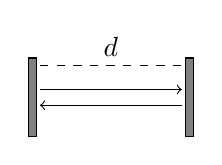
\begin{tikzpicture}
    \draw [fill=gray] (-0.05, -0.5) rectangle (0.05, 0.5);
    \draw [fill=gray] (1.95, -0.5) rectangle (2.05, 0.5);
    \draw [dashed] (0.1, 0.4) -- (1.9, 0.4) node [pos=0.5, above] {$d$};
    \draw [->] (0.1, 0.1) -- (1.9, 0.1);
    \draw [->] (1.9, -0.1) -- (0.1, -0.1);
  \end{tikzpicture}
\end{center}
From the point of view of an observer moving downwards, by the time light reaches the right mirror, it would have moved down a bit. So $S$ sees
\begin{center}
  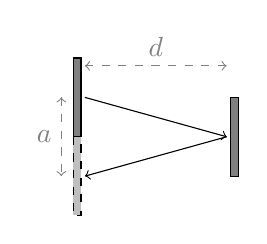
\begin{tikzpicture}
    \draw [fill=gray] (-0.05, -0.5) rectangle (0.05, 0.5);
    \draw [fill=gray] (1.95, -1) rectangle (2.05, 0);
    \draw [->] (0.1, 0) -- (1.9, -0.5);
    \draw [->] (1.9, -0.5) -- (0.1, -1);
    \draw [fill=gray!50!white, dashed] (-0.05, -0.5) rectangle (0.05, -1.5);
    \draw [gray, dashed, ->] (0.1, 0.4) -- (1.9, 0.4) node [pos=0.5, above] {$d$};
    \draw [gray, ->] (0.101, 0.4) -- (0.1, 0.4);
    \draw [gray, ->, dashed] (-0.2, 0) -- (-0.2, -1) node [pos = 0.5, left] {$a$};
    \draw [gray, ->] (-0.2, -0.01) -- (-0.2, 0);
  \end{tikzpicture}
\end{center}
However, the distance travelled by the light beam is now $\sqrt{(2d)^2 + a^2} > 2d$. Since they agree on the speed of light, it must have taken longer for the clock to receive the reflected light in $S$. So the interval between ticks are longer.

By the principle of relativity, all clocks must measure the same time dilation, or else we can compare the two clocks and know if we are ``moving''.

This is famously evidenced by muons. Their half-life is around 2 microseconds (i.e.\ on average they decay to something else after around 2 microseconds). They are created when cosmic rays bombard the atmosphere. However, even if they travel at the speed of light, 2 microseconds only allows it to travel $600\rmm$, certainly not sufficient to reach the surface of Earth. However, we observe \emph{lots} of muons on Earth. This is because muons are travelling so fast that their clocks run really slowly.

\subsubsection*{The twin paradox}
Consider two twins: Luke and Leia. Luke stays at home. Leia travels at a constant speed $v$ to a distant planet $P$, turns around, and returns at the same speed.

In Luke's frame of reference,
\begin{center}
  \begin{tikzpicture}
    \draw (0, 0) -- (3, 0) node [right] {$x$};
    \draw (0, 0) -- (0, 3.3) node [above] {$ct$};
    \node at (0, 1) [left] {Luke};
    \draw (0, 1.5) -- (-0.1, 1.5) node [left] {$cT$};
    \draw (0, 3) -- (-0.1, 3) node [left] {$2cT$};
    \draw (0, 0) -- (0.5, 1.5) node [pos=0.5, right] {Leia: $x = vt$} node [dot] {} node [right] {$A$ (Leia's arrival)} -- (0, 3) node [dot] {} node [right] {$R$};
  \end{tikzpicture}
\end{center}
Leia's arrival ($A$) at $P$ has coordinates
\[
  (ct, x) = (cT, vT).
\]
The time experienced by Leia on her outward journey is
\[
  T' = \gamma\left(T - \frac{v}{c^2}T\right) = \frac{T}{\gamma}.
\]
By Leia's return $R$, Luke has aged by $2T$, but Leia has aged by $\frac{2T}{\gamma} < 2T$. So she is younger than Luke, because of time dilation.

The paradox is: From Leia's perspective, Luke travelled away from her at speed and the returned, so he should be younger than her!

Why is the problem not symmetric?

We can draw Leia's initial frame of reference in dashed lines:
\begin{center}
  \begin{tikzpicture}
    \draw (0, 0) -- (3, 0) node [right] {$x$};
    \draw (0, 0) -- (0, 3.3) node [above] {$ct$};
    \draw (0, 0) -- (0.5, 1.5) node [pos=0.5, right] {Leia} node [dot] {} node [right] {$A$} -- (0, 3) node [pos=0.5, right] {Han} node [dot] {} node [right] {$R$};
    \draw [dashed] (0.5, 1.5) -- (1, 3) node [above] {$ct'$};
    \draw [dashed] (0, 0) -- (3, 1) node [right] {$x'$};
    \draw [dashed] (0.5, 1.5) -- (0, 1.333) node [left] {$X$};
    \draw [dashed] (0.5, 1.5) -- (0, 1.667) node [left] {$Z$};
  \end{tikzpicture}
\end{center}
In Leia's frame, by the time she arrives at $A$, she has experienced a time $T' = \frac{T}{\gamma}$ as shown above. This event is simultaneous with event $X$ in Leia's frame. Then in Luke's frame, the coordinates of $X$ are
\[
  (ct, x) = \left(\frac{cT'}{\gamma}, 0\right) = \left(\frac{cT}{\gamma^2}, 0\right),
\]
obtained through calculations similar to that above. So Leia thinks Luke has aged less by a factor of $1/\gamma^2$. At this stage, the problem \emph{is} symmetric, and Luke also thinks Leia has aged less by a factor of $1/\gamma^2$.

Things change when Leia turns around and changes frame of reference. To understand this better, suppose Leia meets a friend, Han, who is just leaving $P$ at speed $v$. On his journey back, Han also thinks Luke ages $T/\gamma^2$. But in his frame of reference, his departure is simultaneous with Luke's event $Z$, not $X$, since he has different lines of simultaneity.

So the asymmetry between Luke and Leia occurs when Leia turns around. At this point, she sees Luke age rapidly from $X$ to $Z$.

\subsubsection*{Length contraction}
A rod of length $L'$ is stationary in $S'$. What is its length in $S$?

In $S'$, then length of the rod is the distance between the two ends at the same time. So we have
\begin{center}
  \begin{tikzpicture}
    \draw (0, 0) -- (3, 0) node [right] {$x'$};
    \draw (0, 0) -- (0, 3) node [above] {$ct'$};
    \draw (1.5, 3) -- (1.5, 0) node [below] {$L'$};
    \draw [->] (0, 1.5) -- (1.5, 1.5) node [pos = 0.5, above] {$L'$};
    \draw [->] (1.5, 1.5) -- (0, 1.5);
  \end{tikzpicture}
\end{center}
In $S$, we have
\begin{center}
  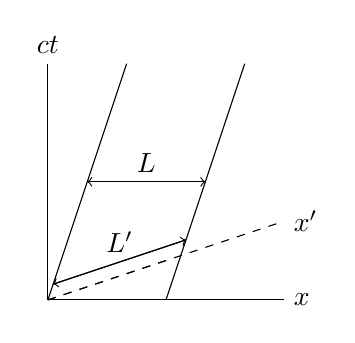
\begin{tikzpicture}
    \draw (0, 0) -- (3, 0) node [right] {$x$};
    \draw (0, 0) -- (0, 3) node [above] {$ct$};
    \draw (0, 0) -- (1, 3);
    \draw (1.5, 0) -- (2.5, 3);
    \draw [->] (0.5, 1.5) -- (2, 1.5) node [pos = 0.5, above] {$L$};
    \draw [->] (2, 1.5) -- (0.5, 1.5);
    \draw [dashed] (0, 0) -- (3, 1) node [right] {$x'$};
    \draw [dashed] (0, 0) -- (1.5, 0.5);
    \draw [->] (0.0667, 0.2) -- (1.75416, 0.7625) node [pos=0.5, above] {$L'$};
    \draw [->] (1.75416, 0.7625) -- (0.0667, 0.2);
  \end{tikzpicture}
\end{center}
The lines $x' = 0$ and $x' = L'$ map into $x = vt$ and $x = vt + L'/\gamma$. So the length in $S$ is $L = L'/\gamma < L'$. Therefore moving objects are contracted in the direction of motion.
\begin{definition}[Proper length]
  The \emph{proper length} is the length measured in an object's rest frame.
\end{definition}

This is analogous to the fact that if you view a bar from an angle, it looks shorter than if you view it from the front. In relativity, what causes the contraction is not a spatial rotation, but a spacetime \emph{hyperbolic} rotation.

Question: does a train of length $2L$ fit alongside a platform of length $L$ if it travels through the station at a speed $v$ such that $\gamma = 2$?

For the system of observers on the platform, the train contracts to a length $2L/\gamma = L$. So it fits.

But for the system of observers on the train, the platform contracts to length $L/\gamma = L/2$, which is much too short!

This can be explained by the difference of lines of simultaneity, since length is the distance between front and back \emph{at the same time}.
\begin{center}
  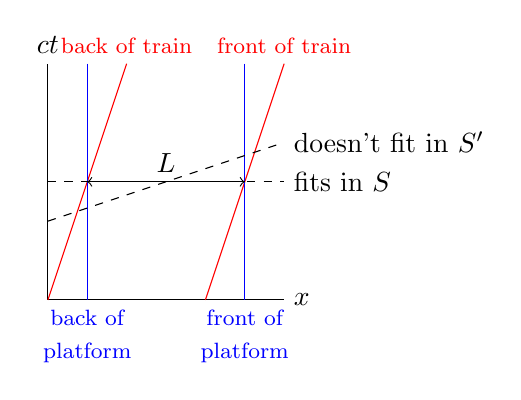
\begin{tikzpicture}
    \draw (0, 0) -- (3, 0) node [right] {$x$};
    \draw (0, 0) -- (0, 3) node [above] {$ct$};
    \draw [red] (0, 0) -- (1, 3) node [above] {\footnotesize back of train};
    \draw [red] (2, 0) -- (3, 3) node [above] {\footnotesize front of train};
    \draw [blue] (0.5, 3) -- (0.5, 0) node [below, align=center] {\footnotesize back of\\\footnotesize platform} ;
    \draw [blue] (2.5, 3) -- (2.5, 0) node [below, align=center] {\footnotesize front of\\\footnotesize platform};
    \draw [->] (0.5, 1.5) -- (2.5, 1.5) node [above, pos=0.5] {$L$};
    \draw [->] (2.5, 1.5) -- (0.5, 1.5);
    \draw [dashed] (0, 1.5) -- (3, 1.5) node [right] {fits in $S$};
    \draw [dashed] (0, 1) -- (3, 2) node [right] {doesn't fit in $S'$};
  \end{tikzpicture}
\end{center}

\subsubsection*{Composition of velocities}
A particle moves with constant velocity $u'$ in frame $S'$, which moves with velocity $v$ relative to $S$. What is its velocity $u$ in $S$?

The world line of the particle in $S'$ is
\[
  x' = u't'.
\]
In $S$, using the inverse Lorentz transformation,
\[
  u = \frac{x}{t} = \frac{\gamma(x' + vt')}{\gamma(t' + (v/c^2) x')} = \frac{u't' + vt'}{t' + (v/c^2)u't'} = \frac{u' + v}{1 + u'v/c^2}.
\]
This is the formula for the relativistic composition of of velocities.

The inverse transformation is found by swapping $u$ and $u'$, and swapping the sign of $v$, i.e.
\[
  u' = \frac{u - v}{1 - uv/c^2}.
\]
Note the following:
\begin{itemize}
  \item if $u'v \ll c^2$, then the transformation reduces to the standard Galilean addition of velocities $u \approx u' + v$.
  \item $u$ is a monotonically increasing function of $u$ for any constant $v$ (with $|v| < c$).
  \item When $u' = \pm c$, $u = u'$ for any $v$, i.e.\ the speed of light is constant in all frames of reference.
  \item Hence $|u'| < c$ iff $|u| < c$. This means that we cannot reach the speed of light by composition of velocities.
\end{itemize}

\subsection{Geometry of spacetime}
We'll now look at the geometry of spacetime, and study the properties of vectors in this spacetime. While spacetime has 4 dimensions, and each point can be represented by 4 real numbers, this is not ordinary $\bbR^4$. This can be seen when changing coordinate systems, instead of rotating the axes like in $\bbR^4$, we ``squash'' the axes towards the diagonal, which is a \emph{hyperbolic rotation}. In particular, we will have a different notion of a dot product. We say that this space has dimension $d = 1 + 3$.

\subsubsection*{The invariant interval}
In regular Euclidean space, given a vector $\mathbf{x}$, all coordinate systems agree on the length $|\mathbf{x}|$. In Minkowski space, they agree on something else.

Consider events $P$ and $Q$ with coordinates $(ct_1, x_1)$ and $(ct_2, x_2)$ separated by $\Delta t = t_2 - t_1$ and $\Delta x = x_2 - x_1$.

\begin{definition}[Invariant interval]
  The \emph{invariant interval} or \emph{spacetime interval} between $P$ and $Q$ is defined as
  \[
    \Delta s^2 = c^2 \Delta t^2 - \Delta x^2.
  \]
  Note that this quantity $\Delta s^2$ can be both positive or negative --- so $\Delta s$ might be imaginary!
\end{definition}

\begin{proposition}
  All inertial observers agree on the value of $\Delta s^2$.
\end{proposition}

\begin{proof}
  \begin{align*}
    c^2 \Delta t'^2 - \Delta x'^2 &= c^2 \gamma^2 \left(\Delta t - \frac{v}{c^2}\Delta x\right)^2 - \gamma^2 (\Delta x - v\Delta t)^2\\
    &= \gamma^2 \left(1 - \frac{v^2}{c^2}\right)(c^2 \Delta t^2 - \Delta x^2)\\
    &= c^2\Delta t^2 - \Delta x^2.\qedhere
  \end{align*}
\end{proof}

In three spatial dimensions,
\[
  \Delta s^2 = c^2\Delta t^2 - \Delta x^2 - \Delta y^2 - \Delta z^2.
\]
We take this as the ``distance'' between the two points. For two infinitesimally separated events, we have
\begin{definition}[Line element]
  The \emph{line element} is
  \[
    \rmd s^2 = c^2 \rmd t^2 - \rmd x^2 - \rmd y^2 - \rmd z^2.
  \]
\end{definition}

\begin{definition}[Timelike, spacelike and lightlike separation]
  Events with $\Delta s^2 > 0$ are \emph{timelike separated}. It is possible to find inertial frames in which the two events occur in the same position, and are purely separated by time. Timelike-separated events lie within each other's light cones and can influence one another.

  Events with $\Delta s^2 < 0$ are \emph{spacelike separated}. It is possible to find inertial frame in which the two events occur in the same time, and are purely separated by space. Spacelike-separated events lie out of each other's light cones and cannot influence one another.

  Events with $\Delta s^2 = 0$ are \emph{lightlike} or \emph{null separated}. In all inertial frames, the events lie on the boundary of each other's light cones. e.g.\ different points in the trajectory of a photon are lightlike separated, hence the name.
\end{definition}
Note that $\Delta s^2 = 0$ does not imply that $P$ and $Q$ are the same event.

\subsubsection*{The Lorentz group}
The coordinates of an event $P$ in frame $S$ can be written as a \emph{4-vector} (i.e.\ 4-component vector) $X$. We write
\[
  X =
  \begin{pmatrix}
    ct\\
    x\\
    y\\
    z
  \end{pmatrix}
\]
The invariant interval between the origin and $P$ can be written as an inner product
\[
  X\cdot X = X^T\eta X = c^2t^2 - x^2 - y^2 - z^2,
\]
where
\[
  \eta =
  \begin{pmatrix}
    1 & 0 & 0 & 0\\
    0 & -1 & 0 & 0\\
    0 & 0 & -1 & 0\\
    0 & 0 & 0 & -1
  \end{pmatrix}.
\]
4-vectors with $X\cdot X > 0$ are called timelike, and those $X \cdot X < 0$ are spacelike. If $X\cdot X = 0$, it is lightlike or null.

A Lorentz transformation is a linear transformation of the coordinates from one frame $S$ to another $S'$, represented by a $4\times 4$ tensor (``matrix''):
\[
  X' = \Lambda X
\]
Lorentz transformations can be defined as those that leave the inner product invariant:
\[
  (\forall X)(X'\cdot X' = X\cdot X),
\]
which implies the matrix equation
\[
  \Lambda^T\eta \Lambda = \eta.\tag{$*$}
\]
These also preserve $X\cdot Y$ if $X$ and $Y$ are both 4-vectors.

Two classes of solution to this equation are:
\[
  \Lambda =
  \begin{pmatrix}
    1 & 0 & 0 & 0\\
    0\\
    0 & & R\\
    0
  \end{pmatrix},
\]
where $R$ is a $3\times 3$ orthogonal matrix, which rotates (or reflects) space and leaves time intact; and
\[
  \Lambda =
  \begin{pmatrix}
    \gamma & -\gamma \beta & 0 & 0\\
    -\gamma\beta & \gamma & 0 & 0\\
    0 & 0 & 1 & 0\\
    0 & 0 & 0 & 1
  \end{pmatrix},
\]
where $\beta = \frac{v}{c}$, and $\gamma = 1/\sqrt{1 - \beta^2}$. Here we leave the $y$ and $z$ coordinates intact, and apply a Lorentz boost along the $x$ direction.

The set of all matrices satisfying equation $(*)$ form the \emph{Lorentz group} $O(1, 3)$. It is generated by rotations and boosts, as defined above, which includes the absurd spatial reflections and time reversal.

The subgroup with $\det \Lambda = +1$ is the \emph{proper Lorentz group} $SO(1, 3)$.

The subgroup that preserves spatial orientation and the direction of time is the \emph{restricted Lorentz group} $SO^+(1, 3)$. Note that this is different from $SO(1, 3)$, since if you do \emph{both} spatial reflection and time reversal, the determinant of the matrix is still positive. We want to eliminate those as well!

\subsubsection*{Rapidity}
Focus on the upper left $2\times 2$ matrix of Lorentz boosts in the $x$ direction. Write
\[
  \Lambda[\beta] =
  \begin{pmatrix}
    \gamma & -\gamma\beta\\
    -\gamma\beta & \gamma
  \end{pmatrix}
  ,\quad
  \gamma = \frac{1}{\sqrt{1 - \beta^2}}.
\]
Combining two boosts in the $x$ direction, we have
\[
  \Lambda[\beta_1]\Lambda[\beta_2] =
  \begin{pmatrix}
    \gamma_1 & -\gamma_1\beta_1\\
    -\gamma_1\beta_1 & \gamma_1
  \end{pmatrix}
  \begin{pmatrix}
    \gamma_2 & -\gamma_2\beta_2\\
    -\gamma_2\beta_2 & \gamma_2
  \end{pmatrix}
  = \Lambda\left[\frac{\beta_1 + \beta_2}{1 + \beta_1\beta_2}\right]
\]
after some messy algebra. This is just the velocity composition formula as before.

This result does not look nice. This suggests that we might be writing things in the wrong way.

We can compare this with spatial rotation. Recall that
\[
  R(\theta) =
  \begin{pmatrix}
    \cos \theta & \sin \theta\\
    -\sin \theta & \cos \theta
  \end{pmatrix}
\]
with
\[
  R(\theta_1)R(\theta_2) = R(\theta_1 + \theta_2).
\]
For Lorentz boosts, we can define
\begin{definition}[Rapidity]
  The \emph{rapidity} of a Lorentz boot is $\phi$ such that
  \[
    \beta = \tanh \phi,\quad \gamma = \cosh\phi,\quad \gamma\beta=\sinh \phi.
  \]
\end{definition}
Then
\[
  \Lambda[\beta] =
  \begin{pmatrix}
    \cosh \phi & -\sinh \phi\\
    -\sinh \phi & \cosh \phi
  \end{pmatrix}
  = \Lambda(\phi).
\]
The rapidities add like rotation angles:
\[
  \Lambda(\phi_1)\Lambda(\phi_2) = \Lambda(\phi_1 + \phi_2).
\]
This shows the close relation betweens spatial rotations and Lorentz boosts. Lorentz boots are simply \emph{hyperbolic} rotations in spacetime!

\subsection{Relativistic kinematics}
In Newtonian mechanics, we describe a particle by its position $\mathbf{x}(t)$, with its velocity being $\mathbf{u}(t) = \frac{\rmd \mathbf{x}}{\rmd t}$.

In relativity, this is unsatisfactory. In special relativity, space and time can be mixed together by Lorentz boosts, and we prefer not to single out time from space. For example, when we write the 4-vector $X$, we put in both the time and space components, and Lorentz transformations are $4\times 4$ matrices that act on $X$.

In the definition of velocity, however, we are differentiating space with respect to time, which is rather weird. First of all, we need something to replace time. Recall that we defined ``proper length'' as the length in the item in its rest frame. Similarly, we can define the \emph{proper time}.

\begin{definition}[Proper time]
  The \emph{proper time} $\tau$ is defined such that
  \[
    \Delta \tau = \frac{\Delta s}{c}
  \]
  $\tau$ is the time experienced by the particle, i.e.\ the time in the particles rest frame.
\end{definition}
The world line of a particle can be parametrized using the proper time by $t(\tau)$ and $\mathbf{x}(\tau)$.
\begin{center}
  \begin{tikzpicture}[yscale=1.3]
    \draw [->] (0, 0) -- (3, 0) node [right] {$x$};
    \draw [->] (0, 0) -- (0, 2.3) node [above] {$ct$};
    \draw (0.7, 0.3) .. controls (0.7, 0.8) and (2, 1.3) .. (2, 1.8);

    \node [dot] at (1.35, 1.05) {};
    \node at (1.35, 1.05) [anchor = north west] {$\tau_1$};
    \node [dot] at (1.93, 1.6) {};
    \node at (1.93, 1.6) [anchor=north west] {$\tau_2$};
  \end{tikzpicture}
\end{center}
Infinitesimal changes are related by
\[
  \rmd \tau = \frac{\rmd s}{c} = \frac{1}{c}\sqrt{c^2\;\rmd t^2 - |\rmd \mathbf{x}|^2} = \sqrt{1 - \frac{|\mathbf{u}|^2}{c^2}}\;\rmd t.
\]
Thus
\[
  \frac{\rmd t}{\rmd \tau} = \gamma_u
\]
with
\[
  \gamma_u = \frac{1}{\sqrt{1 - \frac{|\mathbf{u}|^2}{c^2}}}.
\]
The total time experienced by the particle along a segment of its world line is
\[
  T = \int \;\rmd \tau = \int\frac{1}{\gamma_u}\;\rmd t.
\]
We can then define the \emph{position 4-vector} and \emph{4-velocity}.
\begin{definition}[Position 4-vector and 4-velocty]
  The \emph{position 4-vector} is
  \[
    X(\tau) =
    \begin{pmatrix}
      ct(\tau)\\
      \mathbf{x}(\tau)
    \end{pmatrix}.
  \]
  Its \emph{4-velocity} is defined as
  \[
    U = \frac{\rmd X}{\rmd \tau} =
    \begin{pmatrix}
      c\frac{\rmd t}{\rmd \tau}\\
      \frac{\rmd \mathbf{x}}{\rmd \tau}
    \end{pmatrix}
    = \frac{\rmd t}{\rmd \tau}
    \begin{pmatrix}
      c\\
      \mathbf{u}
    \end{pmatrix} = \gamma_u
    \begin{pmatrix}
      c\\
      \mathbf{u}
    \end{pmatrix},
  \]
  where $\mathbf{u} = \frac{\rmd \mathbf{x}}{\rmd t}$.
\end{definition}
Another common notation is
\[
  X = (ct, \mathbf{x}),\quad U = \gamma_u (c, \mathbf{u}).
\]
If frames $S$ and $S'$ are related by $X' = \Lambda X$, then the 4-velocity also transforms as $U' = \Lambda U$.

\begin{definition}[4-vector]
  A \emph{4-vector} is a 4-component vectors that transforms in this way under a Lorentz transformation, i.e.\ $X' = \Lambda X$.

  When using suffix notation, the indices are written above (superscript) instead of below (subscript). The indices are written with Greek letters which range from $0$ to $3$. So we have $X^\mu$ instead of $X_i$, for $\mu = 0, 1, 2, 3$. If we write $X_\mu$ instead, it means a different thing. This will be explained more in-depth in the electromagnetism course (and you'll get more confused!).
\end{definition}

$U$ is a 4-vector because $X$ is a 4-vector and $\tau$ is a Lorentz invariant. Note that $\rmd X/\rmd t$ is \emph{not} a 4-vector.

Note that this definition of 4-vector is analogous to that of a tensor --- things that transform nicely according to our rules. Then $\tau$ would be a scalar, i.e.\ rank-0 tensor, while $t$ is just a number, not a scalar.

For any 4-vector $U$, the inner product $U\cdot U = U' \cdot U'$ is Lorentz invariant, i.e.\ the same in all inertial frames. In the rest frame of the particle, $U = (c, 0)$. So $U\cdot U = c^2$.

In any other frame, $Y = \gamma_u(c, \mathbf{u})$. So
\[
  Y\cdot Y = \gamma_u^2 (c^2 - |\mathbf{u}|^2) = c^2
\]
as expected.

\subsubsection*{Transformation of velocities revisited}
We have seen that velocities cannot be simply added in relativity. However, the 4-velocity does transform linearly, according to the Lorentz transform:
\[
  U' = \Lambda U.
\]
In frame $S$, consider a particle moving with speed $u$ at an angle $\theta$ to the $x$ axis in the $xy$ plane. This is the most general case for motion not parallel to the Lorentz boost.

Its 4-velocity is
\[
  U =
  \begin{pmatrix}
    \gamma_u c\\
    \gamma_u u\cos \theta\\
    \gamma_u u\sin \theta\\
    0
  \end{pmatrix}, \quad \gamma_u = \frac{1}{\sqrt{1 - u^2/c^2}}.
\]
With frames $S$ and $S'$ in standard configuration (i.e.\ origin coincide at $t = 0$, $S'$ moving in $x$ direction with velocity $v$ relative to $S$),
\[
  U' = \begin{pmatrix}
    \gamma_{u'} c\\
    \gamma_{u'} u'\cos \theta'\\
    \gamma_{u'} u'\sin \theta'\\
    0
  \end{pmatrix}
  =
  \begin{pmatrix}
    \gamma_v & -\gamma_v v/c & 0 & 0\\
    -\gamma_{v} v/c & \gamma_v & 0 & 0\\
    0 & 0 & 1 & 0\\
    0 & 0 & 0 & 1
  \end{pmatrix}
  \begin{pmatrix}
    \gamma_u c\\
    \gamma_u u\cos \theta\\
    \gamma_u u\sin \theta\\
    0
  \end{pmatrix}
\]
Instead of evaluating the whole matrix, we can divide different rows to get useful results.

The ratio of the first two lines gives
\[
  u'\cos \theta' = \frac{u\cos \theta - v}{1 - \frac{uv}{c^2}\cos \theta},
\]
just like the composition of parallel velocities.

The ratio of the third to second line gives
\[
  \tan \theta' = \frac{u\sin \theta}{\gamma_v(u\cos \theta - v)},
\]
which describes \emph{aberration}, a change in the direction of motion of a particle due to the motion of the observer. Note that this isn't just a relativistic effect! If you walk in the rain, you have to hold your umbrella obliquely since the rain seems to you that they are coming from an angle. The relativistic part is the $\gamma_v$ factor in the denominator.

This is also seen in the aberration of starlight ($u = c$) due to the Earth's orbital motion. This causes small annual changes in the apparent positions of stars.
\subsubsection*{4-momentum}
\begin{definition}[4-momentum]
  The \emph{4-momentum} of a particle of mass $m$ is
  \[
    P = mU = m\gamma_u
    \begin{pmatrix}
      c\\
      \mathbf{u}
    \end{pmatrix}
  \]
  The 4-momentum of a system of particles is the sum of the 4-momentum of the particles, and is conserved in the absence of external forces.

  The spatial components of $P$ are the \emph{relativistic 3-momentum},
  \[
    \mathbf{p} = m\gamma_u \mathbf{u},
  \]
  which differs from the Newtonian expression by a factor of $\gamma_u$. Note that $|\mathbf{p}| \to \infty$ as $|\mathbf{u}| \to c$.
\end{definition}

What is the interpretation of the time component $P^0$ (i.e.\ the first time component of the $P$ vector)? We expand for $|\mathbf{u}| \ll c$:
\[
  P^0 = m\gamma c = \frac{mc}{\sqrt{1 - |\mathbf{u}|^2/c^2}} = \frac{1}{c}\left(mc^2 + \frac{1}{2}m|\mathbf{u}|^2 + \cdots\right).
\]
We have a constant term $mc^2$ plus a kinetic energy term $\frac{1}{2}m|\mathbf{u}|^2$, plus more tiny terms, all divided by $c$. So this suggests that $P^0$ is indeed the energy for a particle, and the remaining $\cdots$ terms are relativistic corrections for our old formula $\frac{1}{2}m|\mathbf{u}|^2$ (the $mc^2$ term will be explained later). So we interpret $P$ as
\[
  P =
  \begin{pmatrix}
    E/c\\
    \mathbf{p}
  \end{pmatrix}
\]
\begin{definition}[Relativistic energy]
  The \emph{relativistic energy} of a particle is $E = P^0c$. So
  \[
    E = m\gamma c^2 = mc^2 + \frac{1}{2}m|\mathbf{u}|^2 + \cdots
  \]
\end{definition}
Note that $E\to \infty$ as $|\mathbf{u}| \to c$.

For a stationary particle, we obtain
\[
  E = mc^2.
\]
This implies that mass is a form of energy. $m$ is sometimes called the \emph{rest mass}.

The energy of a moving particle, $m\gamma_u c^2$, is the sum of the rest energy $mc^2$ and kinetic energy $m(\gamma_u - 1)c^2$.

Since $P\cdot P = \frac{E^2}{c^2} - |\mathbf{p}|^2$ is a Lorentz invariant (lengths of 4-vectors are always Lorentz invariant) and equals $m^2 c^2$ in the particle's rest frame, we have the general relation between energy and momentum
\[
  E^2 = |\mathbf{p}|^2 c^2 + m^2c^4
\]
In Newtonian physics, mass and energy are separately conserved. In relativity, mass is not conserved. Instead, it is just another form of energy, and the total energy, including mass energy, is conserved.

Mass can be converged into kinetic energy and vice versa (e.g.\ atomic bombs!)

\subsubsection*{Massless particles}
Particles with zero mass ($m = 0$), e.g.\ photons, can have non-zero momentum and energy because they travel at the speed of light ($\gamma = \infty$).

In this case, $P\cdot P = 0$. So massless particles have light-like (or null) trajectories, and no proper time can be defined for such particles.

Other massless particles in the Standard Model of particle physics include the gluon.

For these particles, energy and momentum are related by
\[
  E^2 = |\mathbf{p}|^2 c^2.
\]
So
\[
  E = |\mathbf{p}|c.
\]
Thus
\[
  P = \frac{E}{c}
  \begin{pmatrix}
    1\\
    \mathbf{n}
  \end{pmatrix},
\]
where $\mathbf{n}$ is a unit (3-)vector in the direction of propagation.

According to quantum mechanics, fundamental ``particles'' aren't really particles but have both particle-like and wave-like properties (if that sounds confusing, yes it is!). Hence we can assign it a \emph{de Broglie wavelength}, according to the \emph{de Broglie relation}:
\[
  |\mathbf{p}| = \frac{h}{\lambda}
\]
where $h \approx 6.63e-34\mathrm{m}^2 \mathrm{kgs}^{-1}$ is \emph{Planck's constant}.

For massless particles, this is consistent with \emph{Planck's relation}:
\[
  E = \frac{hc}{\lambda} = h\nu,
\]
where $\nu = \frac{c}{\lambda}$ is the \emph{wave frequency}.
\subsubsection*{Newton's second law in special relativity}
\begin{definition}[4-force]
  The \emph{4-force} is
  \[
    F = \frac{\rmd P}{\rmd \tau}
  \]
\end{definition}
This equation is the relativistic counterpart to Newton's second law.

It is related to the 3-force $\mathbf{F}$ by
\[
  F = \gamma_u
  \begin{pmatrix}
    \mathbf{F}\cdot \mathbf{u}/c\\
    \mathbf{F}
  \end{pmatrix}
\]
Expanding the definition of the 4-force componentwise, we obtain
\[
  \frac{\rmd E}{\rmd \tau} = \gamma_u \mathbf{F}\cdot \mathbf{u} \Rightarrow \frac{\rmd E}{\rmd t} = \mathbf{F}\cdot \mathbf{u}
\]
and
\[
  \frac{\rmd \mathbf{p}}{\rmd \tau} = \gamma_u \mathbf{F} \Rightarrow \frac{\rmd \mathbf{p}}{\rmd t} = \mathbf{F}
\]
Equivalently, for a particle of mass $m$,
\[
  F =mA,
\]
where
\[
  A = \frac{\rmd U}{\rmd \tau}
\]
is the 4-acceleration.

We have
\[
  U = \gamma_u
  \begin{pmatrix}
    c\\
    \mathbf{u}
  \end{pmatrix}
\]
So
\[
  A = \gamma_u \frac{\rmd U}{\rmd t} = \gamma_u
  \begin{pmatrix}
    \dot{\gamma}_u c\\
    \gamma_u \mathbf{a} + \dot{\gamma}_u \mathbf{u}.
  \end{pmatrix}
\]
where $\mathbf{\mathbf{a}} = \frac{\rmd \mathbf{u}}{\rmd t}$ and $\dot{\gamma}_u = \gamma_u^3 \frac{\mathbf{a}\cdot \mathbf{u}}{c^2}$.

In the instantaneous rest frame of a particle, $\mathbf{u} = \mathbf{0}$ and $\gamma_u = 1$. So
\[
  U =
  \begin{pmatrix}
    c\\
    \mathbf{0}
  \end{pmatrix}, \quad
  A =
  \begin{pmatrix}
    0\\
    \mathbf{a}
  \end{pmatrix}
\]
Then $\mathbf{U}\cdot \mathbf{A} = 0$. Since this is a Lorentz invariant, we have $\mathbf{U} \cdot \mathbf{A} = 0$ in all frames.

\subsection{Particle physics}
Many problems can be solved using the conservation of 4-momentum,
\[
  P =
  \begin{pmatrix}
    E/c\\
    \mathbf{p}
  \end{pmatrix},
\]
for a system of particles.
\begin{definition}[Center of momentum frame]
  The \emph{center of momentum (CM) frame}, or \emph{zero momentum frame}, is an inertial frame in which the total 3-momentum is $\sum \mathbf{p} = 0$.
\end{definition}
This exists unless the system consists of one or more massless particle moving in a single direction.

\subsubsection*{Particle decay}
A particle of mass $m_1$ decays into two particles of masses $m_2$ and $m_2$.

We have
\[
  P_1 = P_2 + P_3.
\]
i.e.
\begin{align*}
  E_1 &= E_2 + E_3\\
  \mathbf{p}_1 &= \mathbf{p}_2 + \mathbf{p}_3.
\end{align*}
In the CM frame (i.e.\ the rest frame of the original particle),
\begin{align*}
  E_1 = m_1 c^2 &= \sqrt{|\mathbf{p}_2|^2 c^2 + m_2^2c^4} + \sqrt{|\mathbf{p}_3|^2 c^2 + m_2^2 c^4}\\
  &\geq m_2c^2 + m_3 c^2.
\end{align*}
So decay is possible only if
\[
  m_1 \geq m_2 + m_3.
\]
(Recall that mass is not conserved in relativity!)

\begin{example}
  A possible decay path of the Higgs' particle can be written as
  \begin{align*}
    \mathrm{h} &\to \gamma \gamma\\
    \text{Higgs'\ particle} &\to 2\text{ photons}
  \end{align*}
  This is possible by the above criterion, because $m_\mathrm{h} \geq 0$, while $m_\gamma = 0$.

  The full conservation equation is
  \[
    P_\mathrm{h} =
    \begin{pmatrix}
      m_\mathrm{h}c\\
      \mathbf{0}
    \end{pmatrix} =
    P_{\gamma_1} + P_{\gamma_2}
  \]
  So
  \begin{align*}
    \mathbf{p}_{\gamma_1} &= \mathbf{p}_{\gamma_2}\\
    E_{\gamma_1} = E_{\gamma_2} &= \frac{1}{2}m_\mathrm{h} c^2.
  \end{align*}
\end{example}

\subsubsection*{Particle scattering}
When two particles collide and retain heir identities, the total 4-momentum is conserved:
\[
  P_1 + P_2 = P_3 + P_4
\]
In the laboratory frame $S$, suppose that particle 1 travels with speed $u$ and collides with particle 2 (at rest).
\begin{center}
  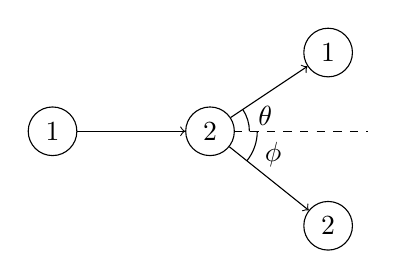
\begin{tikzpicture}
    \node [draw, circle] (1') at (3.5, 1) {1};
    \node [draw, circle] (2') at (3.5, -1.2) {2};
    \node [draw, circle] (2) at (2, 0) {2}
    edge [->] (1')
    edge [->] (2');
    \node [draw, circle] (1) {1}
    edge [->] (2);
    \draw [dashed] (2.3, 0) -- (4, 0);
    \draw (2.5, 0) arc (0:33.69:0.5);
    \draw (2.6, 0) arc (0:-38.66:0.6);
    \node at (2.8, -0.3) {$\phi$};
    \node at (2.7, 0.2) {$\theta$};
  \end{tikzpicture}
\end{center}
In the CM frame $S'$,
\[
  \mathbf{p}'_1 + \mathbf{p}'_2 = 0 = \mathbf{p}_3' + \mathbf{p}'_4.
\]
Both before and after the collision, the two particles have equal and opposite 3-momentum.
\begin{center}
  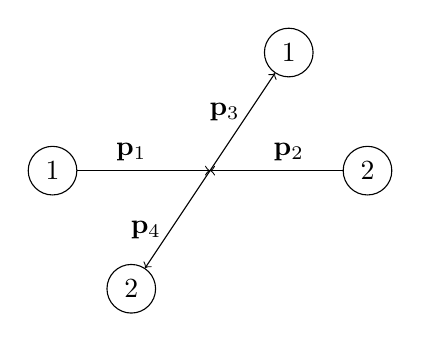
\begin{tikzpicture}
    \node [draw, circle] at (-2, 0) {1}
    edge [->] (0, 0);
    \node [draw, circle] at (2, 0) {2}
    edge [->] (0, 0);
    \node at (-1, 0) [above] {$\mathbf{p}_1$};
    \node at (1, 0) [above] {$\mathbf{p}_2$};
    \node [draw, circle] at (1, 1.5) {1}
    edge [<-] (0, 0);
    \node [draw, circle] at (-1, -1.5) {2}
    edge [<-] (0, 0);
    \node at (0.5, 0.75) [left] {$\mathbf{p}_3$};
    \node at (-0.5, -0.75) [left] {$\mathbf{p}_4$};
  \end{tikzpicture}
\end{center}
The scattering angle $\theta'$ is undetermined and can be thought of as being random. However, we can derive some conclusions about the angles $\theta$ and $\phi$ in the laboratory frame.

(staying in $S'$ for the moment) Suppose the particles have equal mass $m$. They then have the same speed $v$ in $S'$.

Choose axes such that
\[
  P_1' =
  \begin{pmatrix}
    m\gamma_v c\\
    m\gamma_v v\\
    0\\
    0
  \end{pmatrix},\quad
  P_2' =
  \begin{pmatrix}
    m\gamma_v c\\
    -m\gamma_v v\\
    0\\
    0
  \end{pmatrix}
\]
and after the collision,
\[
  P_3' =
  \begin{pmatrix}
    m\gamma_v c\\
    m\gamma_v v\cos \theta'\\
    m\gamma_v v\sin \theta'\\
    0
  \end{pmatrix},\quad
  P_4' =
  \begin{pmatrix}
    m\gamma_v c\\
    -m\gamma_v v\cos \theta'\\
    -m \gamma_v v\sin \theta'\\
    0
  \end{pmatrix}.
\]
We then use the Lorentz transformation to return to the laboratory frame $S$. The relative velocity of the frames is $v$. So the Lorentz transform is
\[
  \Lambda =
  \begin{pmatrix}
    \gamma_v & \gamma_v v/c & 0 & 0\\
    \gamma_v v/c & \gamma_v & 0 & 0\\
    0 & 0 & 1 & 0\\
    0 & 0 & 0 & 1
  \end{pmatrix}
\]
and we find
\[
  P_1 =
  \begin{pmatrix}
    m\gamma_u c\\
    m\gamma_u u\\
    0\\
    0
  \end{pmatrix},\quad
  P_2 =
  \begin{pmatrix}
    mc\\
    0\\
    0\\
    0
  \end{pmatrix}
\]
where
\[
  u = \frac{2v}{1 + v^2/c^2},
\]
(cf.\ velocity composition formula)

Considering the transformations of $P_3'$ and $P_4'$, we obtain
\[
  \tan \theta = \frac{\sin \theta'}{\gamma_v (1 + \cos \theta')} = \frac{1}{\gamma_v}\tan \frac{\theta'}{2},
\]
and
\[
  \tan \phi = \frac{\sin \theta'}{\gamma_v(1 - \cos \theta')} = \frac{1}{\gamma_v}\cot \frac{\theta'}{2}.
\]
Multiplying these expressions together, we obtain
\[
  \tan \theta\tan \phi = \frac{1}{\gamma_v^2}.
\]
So even though we do not know what $\theta$ and $\phi$ might be, they \emph{must} be related by this equation.

In the Newtonian limit, where $|\mathbf{v}| \ll c$, we have $\gamma_v \approx 1$. So
\[
  \tan \theta\tan \phi = 1,
\]
i.e.\ the outgoing trajectories are perpendicular in $S$.

\subsubsection*{Particle creation}
Collide two particles of mass $m$ fast enough, and you create an extra particle of mass $M$.
\[
  P_1 + P_2 = P_3 + P_4 + P_5,
\]
where $P_5$ is the momentum of the new particle.

In the CM frame,
\begin{center}
  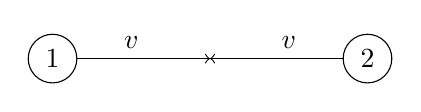
\begin{tikzpicture}
    \node [draw, circle] at (-2, 0) {1}
    edge [->] (0, 0);
    \node [draw, circle] at (2, 0) {2}
    edge [->] (0, 0);
    \node at (-1, 0) [above] {$v$};
    \node at (1, 0) [above] {$v$};
  \end{tikzpicture}
\end{center}
\[
  P_1 + P_2 =
  \begin{pmatrix}
    2m\gamma_v c\\
    \mathbf{0}
  \end{pmatrix}
\]
We have
\[
  P_3 + P_4 + P_5 =
  \begin{pmatrix}
    (E_3 + E_4 + E_5)/c\\
    \mathbf{0}
  \end{pmatrix}
\]
So
\[
  2m\gamma_v c^2 = E_3 + E_4 + E_5 \geq 2mc^2 + Mc^2.
\]
So in order to create this new particle, we must have
\[
  \gamma_v \geq 1 + \frac{M}{2m}.
\]
Alternatively, it occurs only if the initial kinetic energy in the CM frame satisfies
\[
  2(\gamma_v - 1)mc^2 \geq Mc^2.
\]
If we transform to a frame in which the initial speeds are $u$ and 0 (i.e.\ stationary target), then
\[
  u = \frac{2v}{1 + v^2/c^2}
\]
Then
\[
  \gamma_u = 2\gamma_v^2 - 1.
\]
So we require
\[
  \gamma_u \geq 2\left(1 + \frac{M}{2m}\right)^2 - 1 = 1 + \frac{2M}{m} + \frac{M^2}{2m}.
\]
This means that the initial kinetic energy in this frame must be
\[
  m(\gamma_u - 1)c^2 \geq \left(2 + \frac{M}{2m}\right)Mc^2,
\]
which could be much larger than $Mc^2$, especially if $M\gg m$, which usually the case. For example, the mass of the Higgs' boson is 130 times the mass of the proton. So it would be much advantageous to collide two beams of protons head on, as opposed to hitting a fixed target.